\documentclass[twoside]{book}

% Packages required by doxygen
\usepackage{fixltx2e}
\usepackage{calc}
\usepackage{doxygen}
\usepackage[export]{adjustbox} % also loads graphicx
\usepackage{graphicx}
\usepackage[utf8]{inputenc}
\usepackage{makeidx}
\usepackage{multicol}
\usepackage{multirow}
\PassOptionsToPackage{warn}{textcomp}
\usepackage{textcomp}
\usepackage[nointegrals]{wasysym}
\usepackage[table]{xcolor}

% Font selection
\usepackage[T1]{fontenc}
\usepackage[scaled=.90]{helvet}
\usepackage{courier}
\usepackage{amssymb}
\usepackage{sectsty}
\renewcommand{\familydefault}{\sfdefault}
\allsectionsfont{%
  \fontseries{bc}\selectfont%
  \color{darkgray}%
}
\renewcommand{\DoxyLabelFont}{%
  \fontseries{bc}\selectfont%
  \color{darkgray}%
}
\newcommand{\+}{\discretionary{\mbox{\scriptsize$\hookleftarrow$}}{}{}}

% Page & text layout
\usepackage{geometry}
\geometry{%
  a4paper,%
  top=2.5cm,%
  bottom=2.5cm,%
  left=2.5cm,%
  right=2.5cm%
}
\tolerance=750
\hfuzz=15pt
\hbadness=750
\setlength{\emergencystretch}{15pt}
\setlength{\parindent}{0cm}
\setlength{\parskip}{3ex plus 2ex minus 2ex}
\makeatletter
\renewcommand{\paragraph}{%
  \@startsection{paragraph}{4}{0ex}{-1.0ex}{1.0ex}{%
    \normalfont\normalsize\bfseries\SS@parafont%
  }%
}
\renewcommand{\subparagraph}{%
  \@startsection{subparagraph}{5}{0ex}{-1.0ex}{1.0ex}{%
    \normalfont\normalsize\bfseries\SS@subparafont%
  }%
}
\makeatother

% Headers & footers
\usepackage{fancyhdr}
\pagestyle{fancyplain}
\fancyhead[LE]{\fancyplain{}{\bfseries\thepage}}
\fancyhead[CE]{\fancyplain{}{}}
\fancyhead[RE]{\fancyplain{}{\bfseries\leftmark}}
\fancyhead[LO]{\fancyplain{}{\bfseries\rightmark}}
\fancyhead[CO]{\fancyplain{}{}}
\fancyhead[RO]{\fancyplain{}{\bfseries\thepage}}
\fancyfoot[LE]{\fancyplain{}{}}
\fancyfoot[CE]{\fancyplain{}{}}
\fancyfoot[RE]{\fancyplain{}{\bfseries\scriptsize Generated by Doxygen }}
\fancyfoot[LO]{\fancyplain{}{\bfseries\scriptsize Generated by Doxygen }}
\fancyfoot[CO]{\fancyplain{}{}}
\fancyfoot[RO]{\fancyplain{}{}}
\renewcommand{\footrulewidth}{0.4pt}
\renewcommand{\chaptermark}[1]{%
  \markboth{#1}{}%
}
\renewcommand{\sectionmark}[1]{%
  \markright{\thesection\ #1}%
}

% Indices & bibliography
\usepackage{natbib}
\usepackage[titles]{tocloft}
\setcounter{tocdepth}{3}
\setcounter{secnumdepth}{5}
\makeindex

% Hyperlinks (required, but should be loaded last)
\usepackage{ifpdf}
\ifpdf
  \usepackage[pdftex,pagebackref=true]{hyperref}
\else
  \usepackage[ps2pdf,pagebackref=true]{hyperref}
\fi
\hypersetup{%
  colorlinks=true,%
  linkcolor=blue,%
  citecolor=blue,%
  unicode%
}

% Custom commands
\newcommand{\clearemptydoublepage}{%
  \newpage{\pagestyle{empty}\cleardoublepage}%
}

\usepackage{caption}
\captionsetup{labelsep=space,justification=centering,font={bf},singlelinecheck=off,skip=4pt,position=top}

%===== C O N T E N T S =====

\begin{document}

% Titlepage & ToC
\hypersetup{pageanchor=false,
             bookmarksnumbered=true,
             pdfencoding=unicode
            }
\pagenumbering{roman}
\begin{titlepage}
\vspace*{7cm}
\begin{center}%
{\Large Nexus Z\+IA A\+PI }\\
\vspace*{1cm}
{\large Generated by Doxygen 1.8.11}\\
\end{center}
\end{titlepage}
\clearemptydoublepage
\tableofcontents
\clearemptydoublepage
\pagenumbering{arabic}
\hypersetup{pageanchor=true}

%--- Begin generated contents ---
\chapter{Class Index}
\section{Class List}
Here are the classes, structs, unions and interfaces with brief descriptions\+:\begin{DoxyCompactList}
\item\contentsline{section}{\hyperlink{classDefine}{Define} }{\pageref{classDefine}}{}
\item\contentsline{section}{\hyperlink{classnexusZiaApi_1_1IAPIServer}{nexus\+Zia\+Api\+::\+I\+A\+P\+I\+Server} }{\pageref{classnexusZiaApi_1_1IAPIServer}}{}
\item\contentsline{section}{\hyperlink{classnexusZiaApi_1_1IConfigKey}{nexus\+Zia\+Api\+::\+I\+Config\+Key} }{\pageref{classnexusZiaApi_1_1IConfigKey}}{}
\item\contentsline{section}{\hyperlink{classnexusZiaApi_1_1IHooks}{nexus\+Zia\+Api\+::\+I\+Hooks} }{\pageref{classnexusZiaApi_1_1IHooks}}{}
\item\contentsline{section}{\hyperlink{classnexusZiaApi_1_1IHttpData}{nexus\+Zia\+Api\+::\+I\+Http\+Data} }{\pageref{classnexusZiaApi_1_1IHttpData}}{}
\item\contentsline{section}{\hyperlink{classnexusZiaApi_1_1IHttpHeader}{nexus\+Zia\+Api\+::\+I\+Http\+Header} }{\pageref{classnexusZiaApi_1_1IHttpHeader}}{}
\item\contentsline{section}{\hyperlink{classnexusZiaApi_1_1ILogger}{nexus\+Zia\+Api\+::\+I\+Logger} }{\pageref{classnexusZiaApi_1_1ILogger}}{}
\item\contentsline{section}{\hyperlink{classnexusZiaApi_1_1IModuleConfig}{nexus\+Zia\+Api\+::\+I\+Module\+Config} }{\pageref{classnexusZiaApi_1_1IModuleConfig}}{}
\item\contentsline{section}{\hyperlink{classnexusZiaApi_1_1IModuleCore}{nexus\+Zia\+Api\+::\+I\+Module\+Core} }{\pageref{classnexusZiaApi_1_1IModuleCore}}{}
\end{DoxyCompactList}

\chapter{Class Documentation}
\hypertarget{classDefine}{}\section{Define Class Reference}
\label{classDefine}\index{Define@{Define}}


Collaboration diagram for Define\+:
\nopagebreak
\begin{figure}[H]
\begin{center}
\leavevmode
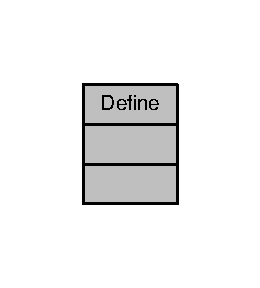
\includegraphics[width=125pt]{classDefine__coll__graph}
\end{center}
\end{figure}


\subsection{Detailed Description}
log 

The documentation for this class was generated from the following file\+:\begin{DoxyCompactItemize}
\item 
/home/convly/delivery/cpp\+\_\+zia\+\_\+api/src/\+Logger/Logger.\+hpp\end{DoxyCompactItemize}

\hypertarget{classnexusZiaApi_1_1IAPIServer}{}\section{nexus\+Zia\+Api\+:\+:I\+A\+P\+I\+Server Class Reference}
\label{classnexusZiaApi_1_1IAPIServer}\index{nexus\+Zia\+Api\+::\+I\+A\+P\+I\+Server@{nexus\+Zia\+Api\+::\+I\+A\+P\+I\+Server}}


Collaboration diagram for nexus\+Zia\+Api\+:\+:I\+A\+P\+I\+Server\+:\nopagebreak
\begin{figure}[H]
\begin{center}
\leavevmode
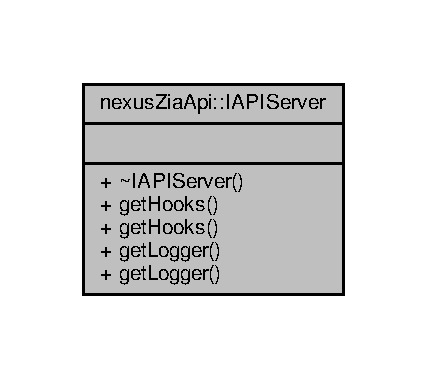
\includegraphics[width=205pt]{classnexusZiaApi_1_1IAPIServer__coll__graph}
\end{center}
\end{figure}
\subsection*{Public Member Functions}
\begin{DoxyCompactItemize}
\item 
virtual \hyperlink{classnexusZiaApi_1_1IHooks}{I\+Hooks} \& \hyperlink{classnexusZiaApi_1_1IAPIServer_ab413ab768d87a8eb41dab45267a54d87}{get\+Hooks} (void)=0
\item 
virtual const \hyperlink{classnexusZiaApi_1_1IHooks}{I\+Hooks} \& \hyperlink{classnexusZiaApi_1_1IAPIServer_aed66cf66c3ccd9f8529a0ea790ae905d}{get\+Hooks} (void) const =0
\item 
virtual \hyperlink{classnexusZiaApi_1_1ILogger}{I\+Logger} \& \hyperlink{classnexusZiaApi_1_1IAPIServer_a534d79505ae46b06c633080cc6fe3fdd}{get\+Logger} (void)=0
\item 
virtual const \hyperlink{classnexusZiaApi_1_1ILogger}{I\+Logger} \& \hyperlink{classnexusZiaApi_1_1IAPIServer_a8304099597c8e182817fbeb66dcb1a59}{get\+Logger} (void) const =0
\end{DoxyCompactItemize}


\subsection{Member Function Documentation}
\index{nexus\+Zia\+Api\+::\+I\+A\+P\+I\+Server@{nexus\+Zia\+Api\+::\+I\+A\+P\+I\+Server}!get\+Hooks@{get\+Hooks}}
\index{get\+Hooks@{get\+Hooks}!nexus\+Zia\+Api\+::\+I\+A\+P\+I\+Server@{nexus\+Zia\+Api\+::\+I\+A\+P\+I\+Server}}
\subsubsection[{\texorpdfstring{get\+Hooks(void)=0}{getHooks(void)=0}}]{\setlength{\rightskip}{0pt plus 5cm}virtual {\bf I\+Hooks}\& nexus\+Zia\+Api\+::\+I\+A\+P\+I\+Server\+::get\+Hooks (
\begin{DoxyParamCaption}
\item[{void}]{}
\end{DoxyParamCaption}
)\hspace{0.3cm}{\ttfamily [pure virtual]}}\hypertarget{classnexusZiaApi_1_1IAPIServer_ab413ab768d87a8eb41dab45267a54d87}{}\label{classnexusZiaApi_1_1IAPIServer_ab413ab768d87a8eb41dab45267a54d87}
Get hooks A\+PI server \begin{DoxyAttention}{Attention}
This functions allow edit of reference 
\end{DoxyAttention}
\begin{DoxyReturn}{Returns}

\end{DoxyReturn}
\index{nexus\+Zia\+Api\+::\+I\+A\+P\+I\+Server@{nexus\+Zia\+Api\+::\+I\+A\+P\+I\+Server}!get\+Hooks@{get\+Hooks}}
\index{get\+Hooks@{get\+Hooks}!nexus\+Zia\+Api\+::\+I\+A\+P\+I\+Server@{nexus\+Zia\+Api\+::\+I\+A\+P\+I\+Server}}
\subsubsection[{\texorpdfstring{get\+Hooks(void) const =0}{getHooks(void) const =0}}]{\setlength{\rightskip}{0pt plus 5cm}virtual const {\bf I\+Hooks}\& nexus\+Zia\+Api\+::\+I\+A\+P\+I\+Server\+::get\+Hooks (
\begin{DoxyParamCaption}
\item[{void}]{}
\end{DoxyParamCaption}
) const\hspace{0.3cm}{\ttfamily [pure virtual]}}\hypertarget{classnexusZiaApi_1_1IAPIServer_aed66cf66c3ccd9f8529a0ea790ae905d}{}\label{classnexusZiaApi_1_1IAPIServer_aed66cf66c3ccd9f8529a0ea790ae905d}
Get hooks A\+PI server \begin{DoxyReturn}{Returns}

\end{DoxyReturn}
\index{nexus\+Zia\+Api\+::\+I\+A\+P\+I\+Server@{nexus\+Zia\+Api\+::\+I\+A\+P\+I\+Server}!get\+Logger@{get\+Logger}}
\index{get\+Logger@{get\+Logger}!nexus\+Zia\+Api\+::\+I\+A\+P\+I\+Server@{nexus\+Zia\+Api\+::\+I\+A\+P\+I\+Server}}
\subsubsection[{\texorpdfstring{get\+Logger(void)=0}{getLogger(void)=0}}]{\setlength{\rightskip}{0pt plus 5cm}virtual {\bf I\+Logger}\& nexus\+Zia\+Api\+::\+I\+A\+P\+I\+Server\+::get\+Logger (
\begin{DoxyParamCaption}
\item[{void}]{}
\end{DoxyParamCaption}
)\hspace{0.3cm}{\ttfamily [pure virtual]}}\hypertarget{classnexusZiaApi_1_1IAPIServer_a534d79505ae46b06c633080cc6fe3fdd}{}\label{classnexusZiaApi_1_1IAPIServer_a534d79505ae46b06c633080cc6fe3fdd}
Get logger A\+PI server \begin{DoxyAttention}{Attention}
This functions allow edit of reference 
\end{DoxyAttention}
\begin{DoxyReturn}{Returns}

\end{DoxyReturn}
\index{nexus\+Zia\+Api\+::\+I\+A\+P\+I\+Server@{nexus\+Zia\+Api\+::\+I\+A\+P\+I\+Server}!get\+Logger@{get\+Logger}}
\index{get\+Logger@{get\+Logger}!nexus\+Zia\+Api\+::\+I\+A\+P\+I\+Server@{nexus\+Zia\+Api\+::\+I\+A\+P\+I\+Server}}
\subsubsection[{\texorpdfstring{get\+Logger(void) const =0}{getLogger(void) const =0}}]{\setlength{\rightskip}{0pt plus 5cm}virtual const {\bf I\+Logger}\& nexus\+Zia\+Api\+::\+I\+A\+P\+I\+Server\+::get\+Logger (
\begin{DoxyParamCaption}
\item[{void}]{}
\end{DoxyParamCaption}
) const\hspace{0.3cm}{\ttfamily [pure virtual]}}\hypertarget{classnexusZiaApi_1_1IAPIServer_a8304099597c8e182817fbeb66dcb1a59}{}\label{classnexusZiaApi_1_1IAPIServer_a8304099597c8e182817fbeb66dcb1a59}
Get logger A\+PI server \begin{DoxyReturn}{Returns}

\end{DoxyReturn}


The documentation for this class was generated from the following file\+:\begin{DoxyCompactItemize}
\item 
/home/convly/delivery/cpp\+\_\+zia\+\_\+api/src/\+Core/A\+P\+I\+Server.\+hpp\end{DoxyCompactItemize}

\hypertarget{classnexusZiaApi_1_1IConfigKey}{}\section{nexus\+Zia\+Api\+:\+:I\+Config\+Key Class Reference}
\label{classnexusZiaApi_1_1IConfigKey}\index{nexus\+Zia\+Api\+::\+I\+Config\+Key@{nexus\+Zia\+Api\+::\+I\+Config\+Key}}


Collaboration diagram for nexus\+Zia\+Api\+:\+:I\+Config\+Key\+:\nopagebreak
\begin{figure}[H]
\begin{center}
\leavevmode
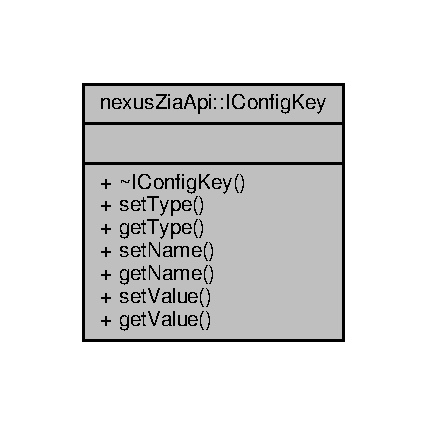
\includegraphics[width=205pt]{classnexusZiaApi_1_1IConfigKey__coll__graph}
\end{center}
\end{figure}
\subsection*{Public Types}
\begin{DoxyCompactItemize}
\item 
enum {\bfseries Type} \{ {\bfseries V\+A\+L\+UE} = 0, 
{\bfseries S\+C\+O\+PE} = 1
 \}\hypertarget{classnexusZiaApi_1_1IConfigKey_a671e0d0f087fe2656476c17378a9778d}{}\label{classnexusZiaApi_1_1IConfigKey_a671e0d0f087fe2656476c17378a9778d}

\end{DoxyCompactItemize}
\subsection*{Public Member Functions}
\begin{DoxyCompactItemize}
\item 
virtual void \hyperlink{classnexusZiaApi_1_1IConfigKey_aef7f67d43c010bdeda6cd1b118eb8a54}{set\+Type} (const Type \&type)=0
\item 
virtual const Type \& \hyperlink{classnexusZiaApi_1_1IConfigKey_a22a271234ecc55dcbe4b978c8c9540a7}{get\+Type} (void) const =0
\item 
virtual void \hyperlink{classnexusZiaApi_1_1IConfigKey_ad3783a5773b75e21ef64f2b7fabb2a4b}{set\+Name} (const std\+::string \&name)=0
\item 
virtual const std\+::string \& \hyperlink{classnexusZiaApi_1_1IConfigKey_ac55ac100276616e04c469f94ad465cd2}{get\+Name} (void) const =0
\item 
virtual void \hyperlink{classnexusZiaApi_1_1IConfigKey_ad0dd9cb4b66d732dd34c57fc72b144e0}{set\+Value} (const std\+::string \&value)=0
\item 
virtual const std\+::string \& \hyperlink{classnexusZiaApi_1_1IConfigKey_a9c45181138c8fac0cf37a7698ba0f2e9}{get\+Value} (void) const =0
\end{DoxyCompactItemize}


\subsection{Member Function Documentation}
\index{nexus\+Zia\+Api\+::\+I\+Config\+Key@{nexus\+Zia\+Api\+::\+I\+Config\+Key}!get\+Name@{get\+Name}}
\index{get\+Name@{get\+Name}!nexus\+Zia\+Api\+::\+I\+Config\+Key@{nexus\+Zia\+Api\+::\+I\+Config\+Key}}
\subsubsection[{\texorpdfstring{get\+Name(void) const =0}{getName(void) const =0}}]{\setlength{\rightskip}{0pt plus 5cm}virtual const std\+::string\& nexus\+Zia\+Api\+::\+I\+Config\+Key\+::get\+Name (
\begin{DoxyParamCaption}
\item[{void}]{}
\end{DoxyParamCaption}
) const\hspace{0.3cm}{\ttfamily [pure virtual]}}\hypertarget{classnexusZiaApi_1_1IConfigKey_ac55ac100276616e04c469f94ad465cd2}{}\label{classnexusZiaApi_1_1IConfigKey_ac55ac100276616e04c469f94ad465cd2}
Get name of config key \begin{DoxyReturn}{Returns}

\end{DoxyReturn}
\index{nexus\+Zia\+Api\+::\+I\+Config\+Key@{nexus\+Zia\+Api\+::\+I\+Config\+Key}!get\+Type@{get\+Type}}
\index{get\+Type@{get\+Type}!nexus\+Zia\+Api\+::\+I\+Config\+Key@{nexus\+Zia\+Api\+::\+I\+Config\+Key}}
\subsubsection[{\texorpdfstring{get\+Type(void) const =0}{getType(void) const =0}}]{\setlength{\rightskip}{0pt plus 5cm}virtual const Type\& nexus\+Zia\+Api\+::\+I\+Config\+Key\+::get\+Type (
\begin{DoxyParamCaption}
\item[{void}]{}
\end{DoxyParamCaption}
) const\hspace{0.3cm}{\ttfamily [pure virtual]}}\hypertarget{classnexusZiaApi_1_1IConfigKey_a22a271234ecc55dcbe4b978c8c9540a7}{}\label{classnexusZiaApi_1_1IConfigKey_a22a271234ecc55dcbe4b978c8c9540a7}
Get type of config key \begin{DoxyReturn}{Returns}

\end{DoxyReturn}
\index{nexus\+Zia\+Api\+::\+I\+Config\+Key@{nexus\+Zia\+Api\+::\+I\+Config\+Key}!get\+Value@{get\+Value}}
\index{get\+Value@{get\+Value}!nexus\+Zia\+Api\+::\+I\+Config\+Key@{nexus\+Zia\+Api\+::\+I\+Config\+Key}}
\subsubsection[{\texorpdfstring{get\+Value(void) const =0}{getValue(void) const =0}}]{\setlength{\rightskip}{0pt plus 5cm}virtual const std\+::string\& nexus\+Zia\+Api\+::\+I\+Config\+Key\+::get\+Value (
\begin{DoxyParamCaption}
\item[{void}]{}
\end{DoxyParamCaption}
) const\hspace{0.3cm}{\ttfamily [pure virtual]}}\hypertarget{classnexusZiaApi_1_1IConfigKey_a9c45181138c8fac0cf37a7698ba0f2e9}{}\label{classnexusZiaApi_1_1IConfigKey_a9c45181138c8fac0cf37a7698ba0f2e9}
Get value of config key \begin{DoxyAttention}{Attention}
Return \char`\"{}\char`\"{} for scope 
\end{DoxyAttention}
\begin{DoxyReturn}{Returns}

\end{DoxyReturn}
\index{nexus\+Zia\+Api\+::\+I\+Config\+Key@{nexus\+Zia\+Api\+::\+I\+Config\+Key}!set\+Name@{set\+Name}}
\index{set\+Name@{set\+Name}!nexus\+Zia\+Api\+::\+I\+Config\+Key@{nexus\+Zia\+Api\+::\+I\+Config\+Key}}
\subsubsection[{\texorpdfstring{set\+Name(const std\+::string \&name)=0}{setName(const std::string &name)=0}}]{\setlength{\rightskip}{0pt plus 5cm}virtual void nexus\+Zia\+Api\+::\+I\+Config\+Key\+::set\+Name (
\begin{DoxyParamCaption}
\item[{const std\+::string \&}]{name}
\end{DoxyParamCaption}
)\hspace{0.3cm}{\ttfamily [pure virtual]}}\hypertarget{classnexusZiaApi_1_1IConfigKey_ad3783a5773b75e21ef64f2b7fabb2a4b}{}\label{classnexusZiaApi_1_1IConfigKey_ad3783a5773b75e21ef64f2b7fabb2a4b}
Set name of config key 
\begin{DoxyParams}{Parameters}
{\em type} & \\
\hline
\end{DoxyParams}
\index{nexus\+Zia\+Api\+::\+I\+Config\+Key@{nexus\+Zia\+Api\+::\+I\+Config\+Key}!set\+Type@{set\+Type}}
\index{set\+Type@{set\+Type}!nexus\+Zia\+Api\+::\+I\+Config\+Key@{nexus\+Zia\+Api\+::\+I\+Config\+Key}}
\subsubsection[{\texorpdfstring{set\+Type(const Type \&type)=0}{setType(const Type &type)=0}}]{\setlength{\rightskip}{0pt plus 5cm}virtual void nexus\+Zia\+Api\+::\+I\+Config\+Key\+::set\+Type (
\begin{DoxyParamCaption}
\item[{const Type \&}]{type}
\end{DoxyParamCaption}
)\hspace{0.3cm}{\ttfamily [pure virtual]}}\hypertarget{classnexusZiaApi_1_1IConfigKey_aef7f67d43c010bdeda6cd1b118eb8a54}{}\label{classnexusZiaApi_1_1IConfigKey_aef7f67d43c010bdeda6cd1b118eb8a54}
Set type of config key 
\begin{DoxyParams}{Parameters}
{\em type} & \\
\hline
\end{DoxyParams}
\index{nexus\+Zia\+Api\+::\+I\+Config\+Key@{nexus\+Zia\+Api\+::\+I\+Config\+Key}!set\+Value@{set\+Value}}
\index{set\+Value@{set\+Value}!nexus\+Zia\+Api\+::\+I\+Config\+Key@{nexus\+Zia\+Api\+::\+I\+Config\+Key}}
\subsubsection[{\texorpdfstring{set\+Value(const std\+::string \&value)=0}{setValue(const std::string &value)=0}}]{\setlength{\rightskip}{0pt plus 5cm}virtual void nexus\+Zia\+Api\+::\+I\+Config\+Key\+::set\+Value (
\begin{DoxyParamCaption}
\item[{const std\+::string \&}]{value}
\end{DoxyParamCaption}
)\hspace{0.3cm}{\ttfamily [pure virtual]}}\hypertarget{classnexusZiaApi_1_1IConfigKey_ad0dd9cb4b66d732dd34c57fc72b144e0}{}\label{classnexusZiaApi_1_1IConfigKey_ad0dd9cb4b66d732dd34c57fc72b144e0}
Set value of config key \begin{DoxyAttention}{Attention}
Not for scope type 
\end{DoxyAttention}

\begin{DoxyParams}{Parameters}
{\em type} & \\
\hline
\end{DoxyParams}


The documentation for this class was generated from the following file\+:\begin{DoxyCompactItemize}
\item 
/home/convly/delivery/cpp\+\_\+zia\+\_\+api/src/\+Config/Config\+Key.\+hpp\end{DoxyCompactItemize}

\hypertarget{classnexusZiaApi_1_1IHooks}{}\section{nexus\+Zia\+Api\+:\+:I\+Hooks Class Reference}
\label{classnexusZiaApi_1_1IHooks}\index{nexus\+Zia\+Api\+::\+I\+Hooks@{nexus\+Zia\+Api\+::\+I\+Hooks}}


Collaboration diagram for nexus\+Zia\+Api\+:\+:I\+Hooks\+:\nopagebreak
\begin{figure}[H]
\begin{center}
\leavevmode
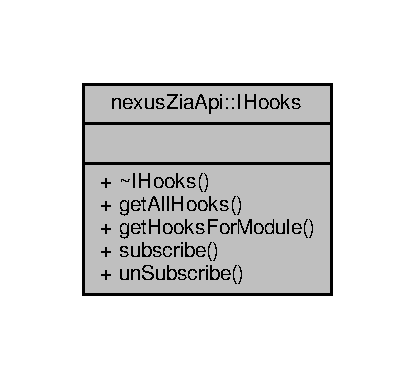
\includegraphics[width=199pt]{classnexusZiaApi_1_1IHooks__coll__graph}
\end{center}
\end{figure}
\subsection*{Public Types}
\begin{DoxyCompactItemize}
\item 
enum \hyperlink{classnexusZiaApi_1_1IHooks_ab414a80fd9ed1c967916942ec5c20433}{Types} \{ \\*
{\bfseries D\+E\+F\+A\+U\+LT} = 0, 
{\bfseries R\+E\+Q\+U\+E\+S\+T\+\_\+\+B\+E\+F\+O\+R\+E\+\_\+\+P\+A\+R\+S\+I\+NG} = 1, 
{\bfseries R\+E\+Q\+U\+E\+S\+T\+\_\+\+A\+F\+T\+E\+R\+\_\+\+P\+A\+R\+S\+I\+NG} = 2, 
{\bfseries R\+E\+Q\+U\+E\+S\+T\+\_\+\+D\+O\+NE} = 3, 
\\*
{\bfseries R\+E\+S\+P\+O\+N\+S\+E\+\_\+\+B\+E\+F\+O\+R\+E\+\_\+\+B\+U\+I\+LD} = 4, 
{\bfseries R\+E\+S\+P\+O\+N\+S\+E\+\_\+\+P\+O\+S\+T\+\_\+\+B\+U\+I\+LD} = 5, 
{\bfseries R\+E\+S\+P\+O\+N\+S\+E\+\_\+\+S\+E\+ND} = 6
 \}
\end{DoxyCompactItemize}
\subsection*{Public Member Functions}
\begin{DoxyCompactItemize}
\item 
virtual const std\+::list$<$ \hyperlink{classnexusZiaApi_1_1IHooks_ab414a80fd9ed1c967916942ec5c20433}{Types} $>$ \& \hyperlink{classnexusZiaApi_1_1IHooks_a5e372c9b2564fad0f883657ebff2cc73}{get\+All\+Hooks} (void) const =0
\item 
virtual const std\+::list$<$ \hyperlink{classnexusZiaApi_1_1IHooks_ab414a80fd9ed1c967916942ec5c20433}{Types} $>$ \& \hyperlink{classnexusZiaApi_1_1IHooks_ab5e5eac6628b89fed36fcbc0586cfd88}{get\+Hooks\+For\+Module} (const std\+::string \&name) const =0
\item 
virtual void \hyperlink{classnexusZiaApi_1_1IHooks_a389e3429bc6e80f3583c5616e52dcfbe}{subscribe} (const \hyperlink{classnexusZiaApi_1_1IHooks_ab414a80fd9ed1c967916942ec5c20433}{Types} \&type, const std\+::string \&name)=0
\item 
virtual void \hyperlink{classnexusZiaApi_1_1IHooks_a9603e6d03b818729c1c1cf17a090bf0a}{un\+Subscribe} (const \hyperlink{classnexusZiaApi_1_1IHooks_ab414a80fd9ed1c967916942ec5c20433}{Types} \&type, const std\+::string \&name)=0
\end{DoxyCompactItemize}


\subsection{Member Enumeration Documentation}
\index{nexus\+Zia\+Api\+::\+I\+Hooks@{nexus\+Zia\+Api\+::\+I\+Hooks}!Types@{Types}}
\index{Types@{Types}!nexus\+Zia\+Api\+::\+I\+Hooks@{nexus\+Zia\+Api\+::\+I\+Hooks}}
\subsubsection[{\texorpdfstring{Types}{Types}}]{\setlength{\rightskip}{0pt plus 5cm}enum {\bf nexus\+Zia\+Api\+::\+I\+Hooks\+::\+Types}\hspace{0.3cm}{\ttfamily [strong]}}\hypertarget{classnexusZiaApi_1_1IHooks_ab414a80fd9ed1c967916942ec5c20433}{}\label{classnexusZiaApi_1_1IHooks_ab414a80fd9ed1c967916942ec5c20433}
\hyperlink{classDefine}{Define} type of hook define 

\subsection{Member Function Documentation}
\index{nexus\+Zia\+Api\+::\+I\+Hooks@{nexus\+Zia\+Api\+::\+I\+Hooks}!get\+All\+Hooks@{get\+All\+Hooks}}
\index{get\+All\+Hooks@{get\+All\+Hooks}!nexus\+Zia\+Api\+::\+I\+Hooks@{nexus\+Zia\+Api\+::\+I\+Hooks}}
\subsubsection[{\texorpdfstring{get\+All\+Hooks(void) const =0}{getAllHooks(void) const =0}}]{\setlength{\rightskip}{0pt plus 5cm}virtual const std\+::list$<${\bf Types}$>$\& nexus\+Zia\+Api\+::\+I\+Hooks\+::get\+All\+Hooks (
\begin{DoxyParamCaption}
\item[{void}]{}
\end{DoxyParamCaption}
) const\hspace{0.3cm}{\ttfamily [pure virtual]}}\hypertarget{classnexusZiaApi_1_1IHooks_a5e372c9b2564fad0f883657ebff2cc73}{}\label{classnexusZiaApi_1_1IHooks_a5e372c9b2564fad0f883657ebff2cc73}
Get list of hooks \begin{DoxyReturn}{Returns}

\end{DoxyReturn}
\index{nexus\+Zia\+Api\+::\+I\+Hooks@{nexus\+Zia\+Api\+::\+I\+Hooks}!get\+Hooks\+For\+Module@{get\+Hooks\+For\+Module}}
\index{get\+Hooks\+For\+Module@{get\+Hooks\+For\+Module}!nexus\+Zia\+Api\+::\+I\+Hooks@{nexus\+Zia\+Api\+::\+I\+Hooks}}
\subsubsection[{\texorpdfstring{get\+Hooks\+For\+Module(const std\+::string \&name) const =0}{getHooksForModule(const std::string &name) const =0}}]{\setlength{\rightskip}{0pt plus 5cm}virtual const std\+::list$<${\bf Types}$>$\& nexus\+Zia\+Api\+::\+I\+Hooks\+::get\+Hooks\+For\+Module (
\begin{DoxyParamCaption}
\item[{const std\+::string \&}]{name}
\end{DoxyParamCaption}
) const\hspace{0.3cm}{\ttfamily [pure virtual]}}\hypertarget{classnexusZiaApi_1_1IHooks_ab5e5eac6628b89fed36fcbc0586cfd88}{}\label{classnexusZiaApi_1_1IHooks_ab5e5eac6628b89fed36fcbc0586cfd88}
Get hooks register for module (by name) 
\begin{DoxyParams}{Parameters}
{\em name} & Module name \\
\hline
\end{DoxyParams}
\begin{DoxyReturn}{Returns}

\end{DoxyReturn}
\index{nexus\+Zia\+Api\+::\+I\+Hooks@{nexus\+Zia\+Api\+::\+I\+Hooks}!subscribe@{subscribe}}
\index{subscribe@{subscribe}!nexus\+Zia\+Api\+::\+I\+Hooks@{nexus\+Zia\+Api\+::\+I\+Hooks}}
\subsubsection[{\texorpdfstring{subscribe(const Types \&type, const std\+::string \&name)=0}{subscribe(const Types &type, const std::string &name)=0}}]{\setlength{\rightskip}{0pt plus 5cm}virtual void nexus\+Zia\+Api\+::\+I\+Hooks\+::subscribe (
\begin{DoxyParamCaption}
\item[{const {\bf Types} \&}]{type, }
\item[{const std\+::string \&}]{name}
\end{DoxyParamCaption}
)\hspace{0.3cm}{\ttfamily [pure virtual]}}\hypertarget{classnexusZiaApi_1_1IHooks_a389e3429bc6e80f3583c5616e52dcfbe}{}\label{classnexusZiaApi_1_1IHooks_a389e3429bc6e80f3583c5616e52dcfbe}
Add hook register 
\begin{DoxyParams}{Parameters}
{\em type} & Type hooks \\
\hline
{\em name} & Name of module \\
\hline
\end{DoxyParams}
\index{nexus\+Zia\+Api\+::\+I\+Hooks@{nexus\+Zia\+Api\+::\+I\+Hooks}!un\+Subscribe@{un\+Subscribe}}
\index{un\+Subscribe@{un\+Subscribe}!nexus\+Zia\+Api\+::\+I\+Hooks@{nexus\+Zia\+Api\+::\+I\+Hooks}}
\subsubsection[{\texorpdfstring{un\+Subscribe(const Types \&type, const std\+::string \&name)=0}{unSubscribe(const Types &type, const std::string &name)=0}}]{\setlength{\rightskip}{0pt plus 5cm}virtual void nexus\+Zia\+Api\+::\+I\+Hooks\+::un\+Subscribe (
\begin{DoxyParamCaption}
\item[{const {\bf Types} \&}]{type, }
\item[{const std\+::string \&}]{name}
\end{DoxyParamCaption}
)\hspace{0.3cm}{\ttfamily [pure virtual]}}\hypertarget{classnexusZiaApi_1_1IHooks_a9603e6d03b818729c1c1cf17a090bf0a}{}\label{classnexusZiaApi_1_1IHooks_a9603e6d03b818729c1c1cf17a090bf0a}
Remove hook register 
\begin{DoxyParams}{Parameters}
{\em type} & Type hooks \\
\hline
{\em name} & Name of module \\
\hline
\end{DoxyParams}


The documentation for this class was generated from the following file\+:\begin{DoxyCompactItemize}
\item 
/home/convly/delivery/cpp\+\_\+zia\+\_\+api/src/\+Hooks/Hooks.\+hpp\end{DoxyCompactItemize}

\hypertarget{classnexusZiaApi_1_1IHttpData}{}\section{nexus\+Zia\+Api\+:\+:I\+Http\+Data Class Reference}
\label{classnexusZiaApi_1_1IHttpData}\index{nexus\+Zia\+Api\+::\+I\+Http\+Data@{nexus\+Zia\+Api\+::\+I\+Http\+Data}}


Collaboration diagram for nexus\+Zia\+Api\+:\+:I\+Http\+Data\+:\nopagebreak
\begin{figure}[H]
\begin{center}
\leavevmode
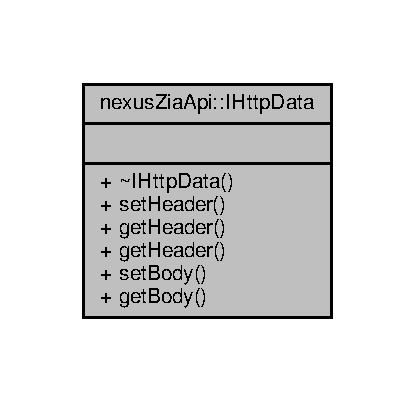
\includegraphics[width=199pt]{classnexusZiaApi_1_1IHttpData__coll__graph}
\end{center}
\end{figure}
\subsection*{Public Member Functions}
\begin{DoxyCompactItemize}
\item 
virtual void \hyperlink{classnexusZiaApi_1_1IHttpData_ad53ebfed899c1e965f32501bc63db5c5}{set\+Header} (const \hyperlink{classnexusZiaApi_1_1IHttpHeader}{I\+Http\+Header} \&header) const 
\item 
virtual \hyperlink{classnexusZiaApi_1_1IHttpHeader}{I\+Http\+Header} \& \hyperlink{classnexusZiaApi_1_1IHttpData_a41df45bc96104ac6c03cdbacb6de0bff}{get\+Header} (void)
\item 
virtual const \hyperlink{classnexusZiaApi_1_1IHttpHeader}{I\+Http\+Header} \& \hyperlink{classnexusZiaApi_1_1IHttpData_afce627a46cbc6e85fc0e652ae6814bcd}{get\+Header} (void) const 
\item 
virtual void \hyperlink{classnexusZiaApi_1_1IHttpData_a6f693ebbf8d1e36dc2e05b1c0815c1a7}{set\+Body} (const std\+::string \&data)=0
\item 
virtual const std\+::string \& \hyperlink{classnexusZiaApi_1_1IHttpData_aa591f37edf9e38071e35b2f771eeae1e}{get\+Body} (void) const =0
\end{DoxyCompactItemize}


\subsection{Member Function Documentation}
\index{nexus\+Zia\+Api\+::\+I\+Http\+Data@{nexus\+Zia\+Api\+::\+I\+Http\+Data}!get\+Body@{get\+Body}}
\index{get\+Body@{get\+Body}!nexus\+Zia\+Api\+::\+I\+Http\+Data@{nexus\+Zia\+Api\+::\+I\+Http\+Data}}
\subsubsection[{\texorpdfstring{get\+Body(void) const =0}{getBody(void) const =0}}]{\setlength{\rightskip}{0pt plus 5cm}virtual const std\+::string\& nexus\+Zia\+Api\+::\+I\+Http\+Data\+::get\+Body (
\begin{DoxyParamCaption}
\item[{void}]{}
\end{DoxyParamCaption}
) const\hspace{0.3cm}{\ttfamily [pure virtual]}}\hypertarget{classnexusZiaApi_1_1IHttpData_aa591f37edf9e38071e35b2f771eeae1e}{}\label{classnexusZiaApi_1_1IHttpData_aa591f37edf9e38071e35b2f771eeae1e}
Get body of H\+T\+TP Data \begin{DoxyReturn}{Returns}

\end{DoxyReturn}
\index{nexus\+Zia\+Api\+::\+I\+Http\+Data@{nexus\+Zia\+Api\+::\+I\+Http\+Data}!get\+Header@{get\+Header}}
\index{get\+Header@{get\+Header}!nexus\+Zia\+Api\+::\+I\+Http\+Data@{nexus\+Zia\+Api\+::\+I\+Http\+Data}}
\subsubsection[{\texorpdfstring{get\+Header(void)}{getHeader(void)}}]{\setlength{\rightskip}{0pt plus 5cm}virtual {\bf I\+Http\+Header}\& nexus\+Zia\+Api\+::\+I\+Http\+Data\+::get\+Header (
\begin{DoxyParamCaption}
\item[{void}]{}
\end{DoxyParamCaption}
)\hspace{0.3cm}{\ttfamily [virtual]}}\hypertarget{classnexusZiaApi_1_1IHttpData_a41df45bc96104ac6c03cdbacb6de0bff}{}\label{classnexusZiaApi_1_1IHttpData_a41df45bc96104ac6c03cdbacb6de0bff}
Get H\+T\+TP Header \begin{DoxyAttention}{Attention}
This functions allow edit of reference 
\end{DoxyAttention}
\begin{DoxyReturn}{Returns}

\end{DoxyReturn}
\index{nexus\+Zia\+Api\+::\+I\+Http\+Data@{nexus\+Zia\+Api\+::\+I\+Http\+Data}!get\+Header@{get\+Header}}
\index{get\+Header@{get\+Header}!nexus\+Zia\+Api\+::\+I\+Http\+Data@{nexus\+Zia\+Api\+::\+I\+Http\+Data}}
\subsubsection[{\texorpdfstring{get\+Header(void) const }{getHeader(void) const }}]{\setlength{\rightskip}{0pt plus 5cm}virtual const {\bf I\+Http\+Header}\& nexus\+Zia\+Api\+::\+I\+Http\+Data\+::get\+Header (
\begin{DoxyParamCaption}
\item[{void}]{}
\end{DoxyParamCaption}
) const\hspace{0.3cm}{\ttfamily [virtual]}}\hypertarget{classnexusZiaApi_1_1IHttpData_afce627a46cbc6e85fc0e652ae6814bcd}{}\label{classnexusZiaApi_1_1IHttpData_afce627a46cbc6e85fc0e652ae6814bcd}
Get H\+T\+TP Header \begin{DoxyReturn}{Returns}

\end{DoxyReturn}
\index{nexus\+Zia\+Api\+::\+I\+Http\+Data@{nexus\+Zia\+Api\+::\+I\+Http\+Data}!set\+Body@{set\+Body}}
\index{set\+Body@{set\+Body}!nexus\+Zia\+Api\+::\+I\+Http\+Data@{nexus\+Zia\+Api\+::\+I\+Http\+Data}}
\subsubsection[{\texorpdfstring{set\+Body(const std\+::string \&data)=0}{setBody(const std::string &data)=0}}]{\setlength{\rightskip}{0pt plus 5cm}virtual void nexus\+Zia\+Api\+::\+I\+Http\+Data\+::set\+Body (
\begin{DoxyParamCaption}
\item[{const std\+::string \&}]{data}
\end{DoxyParamCaption}
)\hspace{0.3cm}{\ttfamily [pure virtual]}}\hypertarget{classnexusZiaApi_1_1IHttpData_a6f693ebbf8d1e36dc2e05b1c0815c1a7}{}\label{classnexusZiaApi_1_1IHttpData_a6f693ebbf8d1e36dc2e05b1c0815c1a7}
Set the body of H\+T\+TP Data 
\begin{DoxyParams}{Parameters}
{\em data} & \\
\hline
\end{DoxyParams}
\index{nexus\+Zia\+Api\+::\+I\+Http\+Data@{nexus\+Zia\+Api\+::\+I\+Http\+Data}!set\+Header@{set\+Header}}
\index{set\+Header@{set\+Header}!nexus\+Zia\+Api\+::\+I\+Http\+Data@{nexus\+Zia\+Api\+::\+I\+Http\+Data}}
\subsubsection[{\texorpdfstring{set\+Header(const I\+Http\+Header \&header) const }{setHeader(const IHttpHeader &header) const }}]{\setlength{\rightskip}{0pt plus 5cm}virtual void nexus\+Zia\+Api\+::\+I\+Http\+Data\+::set\+Header (
\begin{DoxyParamCaption}
\item[{const {\bf I\+Http\+Header} \&}]{header}
\end{DoxyParamCaption}
) const\hspace{0.3cm}{\ttfamily [virtual]}}\hypertarget{classnexusZiaApi_1_1IHttpData_ad53ebfed899c1e965f32501bc63db5c5}{}\label{classnexusZiaApi_1_1IHttpData_ad53ebfed899c1e965f32501bc63db5c5}
\hyperlink{classDefine}{Define} header of H\+T\+TP data (or message) 
\begin{DoxyParams}{Parameters}
{\em header} & \\
\hline
\end{DoxyParams}


The documentation for this class was generated from the following file\+:\begin{DoxyCompactItemize}
\item 
/home/convly/delivery/cpp\+\_\+zia\+\_\+api/src/\+Http/Http\+Data.\+hpp\end{DoxyCompactItemize}

\hypertarget{classnexusZiaApi_1_1IHttpHeader}{}\section{nexus\+Zia\+Api\+:\+:I\+Http\+Header Class Reference}
\label{classnexusZiaApi_1_1IHttpHeader}\index{nexus\+Zia\+Api\+::\+I\+Http\+Header@{nexus\+Zia\+Api\+::\+I\+Http\+Header}}


Collaboration diagram for nexus\+Zia\+Api\+:\+:I\+Http\+Header\+:\nopagebreak
\begin{figure}[H]
\begin{center}
\leavevmode
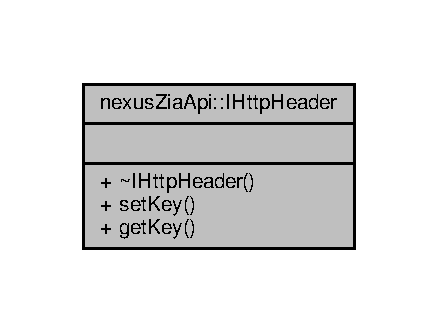
\includegraphics[width=210pt]{classnexusZiaApi_1_1IHttpHeader__coll__graph}
\end{center}
\end{figure}
\subsection*{Public Member Functions}
\begin{DoxyCompactItemize}
\item 
virtual void \hyperlink{classnexusZiaApi_1_1IHttpHeader_ad7bbf7ae0822953c462b2098c24a0eaf}{set\+Key} (const std\+::string \&key, const std\+::string \&value)=0
\item 
virtual const std\+::string \& \hyperlink{classnexusZiaApi_1_1IHttpHeader_a165d7493d3f6a8f2cbb498776c835e87}{get\+Key} (const std\+::string \&key)=0
\end{DoxyCompactItemize}


\subsection{Member Function Documentation}
\index{nexus\+Zia\+Api\+::\+I\+Http\+Header@{nexus\+Zia\+Api\+::\+I\+Http\+Header}!get\+Key@{get\+Key}}
\index{get\+Key@{get\+Key}!nexus\+Zia\+Api\+::\+I\+Http\+Header@{nexus\+Zia\+Api\+::\+I\+Http\+Header}}
\subsubsection[{\texorpdfstring{get\+Key(const std\+::string \&key)=0}{getKey(const std::string &key)=0}}]{\setlength{\rightskip}{0pt plus 5cm}virtual const std\+::string\& nexus\+Zia\+Api\+::\+I\+Http\+Header\+::get\+Key (
\begin{DoxyParamCaption}
\item[{const std\+::string \&}]{key}
\end{DoxyParamCaption}
)\hspace{0.3cm}{\ttfamily [pure virtual]}}\hypertarget{classnexusZiaApi_1_1IHttpHeader_a165d7493d3f6a8f2cbb498776c835e87}{}\label{classnexusZiaApi_1_1IHttpHeader_a165d7493d3f6a8f2cbb498776c835e87}
Get key of header H\+T\+TP 
\begin{DoxyParams}{Parameters}
{\em key} & \\
\hline
\end{DoxyParams}
\begin{DoxyReturn}{Returns}

\end{DoxyReturn}
\index{nexus\+Zia\+Api\+::\+I\+Http\+Header@{nexus\+Zia\+Api\+::\+I\+Http\+Header}!set\+Key@{set\+Key}}
\index{set\+Key@{set\+Key}!nexus\+Zia\+Api\+::\+I\+Http\+Header@{nexus\+Zia\+Api\+::\+I\+Http\+Header}}
\subsubsection[{\texorpdfstring{set\+Key(const std\+::string \&key, const std\+::string \&value)=0}{setKey(const std::string &key, const std::string &value)=0}}]{\setlength{\rightskip}{0pt plus 5cm}virtual void nexus\+Zia\+Api\+::\+I\+Http\+Header\+::set\+Key (
\begin{DoxyParamCaption}
\item[{const std\+::string \&}]{key, }
\item[{const std\+::string \&}]{value}
\end{DoxyParamCaption}
)\hspace{0.3cm}{\ttfamily [pure virtual]}}\hypertarget{classnexusZiaApi_1_1IHttpHeader_ad7bbf7ae0822953c462b2098c24a0eaf}{}\label{classnexusZiaApi_1_1IHttpHeader_ad7bbf7ae0822953c462b2098c24a0eaf}
Set key of header H\+T\+TP 
\begin{DoxyParams}{Parameters}
{\em key} & \\
\hline
{\em value} & \\
\hline
\end{DoxyParams}
\begin{DoxyReturn}{Returns}

\end{DoxyReturn}


The documentation for this class was generated from the following file\+:\begin{DoxyCompactItemize}
\item 
/home/convly/delivery/cpp\+\_\+zia\+\_\+api/src/\+Http/Http\+Header.\+hpp\end{DoxyCompactItemize}

\hypertarget{classnexusZiaApi_1_1ILogger}{}\section{nexus\+Zia\+Api\+:\+:I\+Logger Class Reference}
\label{classnexusZiaApi_1_1ILogger}\index{nexus\+Zia\+Api\+::\+I\+Logger@{nexus\+Zia\+Api\+::\+I\+Logger}}


Collaboration diagram for nexus\+Zia\+Api\+:\+:I\+Logger\+:\nopagebreak
\begin{figure}[H]
\begin{center}
\leavevmode
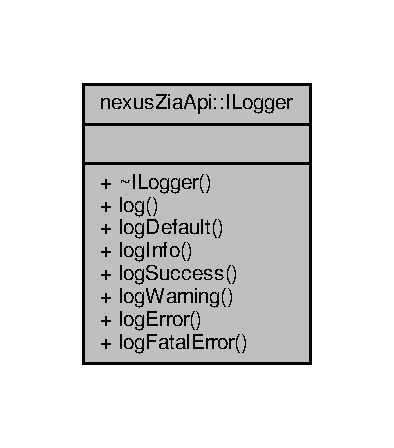
\includegraphics[width=189pt]{classnexusZiaApi_1_1ILogger__coll__graph}
\end{center}
\end{figure}
\subsection*{Public Types}
\begin{DoxyCompactItemize}
\item 
enum {\bfseries Level} \{ \\*
{\bfseries D\+E\+F\+A\+U\+LT} = 0, 
{\bfseries I\+N\+FO} = 1, 
{\bfseries S\+U\+C\+C\+E\+SS} = 2, 
{\bfseries W\+A\+R\+N\+I\+NG} = 3, 
\\*
{\bfseries E\+R\+R\+OR} = 4, 
{\bfseries F\+A\+T\+A\+L\+\_\+\+E\+R\+R\+OR} = 5
 \}\hypertarget{classnexusZiaApi_1_1ILogger_a7e523ee9ecfe0b304c0f43c29fc447b5}{}\label{classnexusZiaApi_1_1ILogger_a7e523ee9ecfe0b304c0f43c29fc447b5}

\end{DoxyCompactItemize}
\subsection*{Public Member Functions}
\begin{DoxyCompactItemize}
\item 
virtual void \hyperlink{classnexusZiaApi_1_1ILogger_a3fdab5380f82bfac1a68d58ae8a3f23d}{log} (const I\+Logger\+::\+Level \&level, const std\+::string \&msg)=0
\item 
virtual void \hyperlink{classnexusZiaApi_1_1ILogger_ae2fe20e82d85ab89f9f67135562c1427}{log\+Default} (const std\+::string \&msg)=0
\item 
virtual void \hyperlink{classnexusZiaApi_1_1ILogger_a3b8b8623cb92ecbe28a6e00e06a2d97d}{log\+Info} (const std\+::string \&msg)=0
\item 
virtual void \hyperlink{classnexusZiaApi_1_1ILogger_a17a3b1b8faadd679b9c15a349a7d8f57}{log\+Success} (const std\+::string \&msg)=0
\item 
virtual void \hyperlink{classnexusZiaApi_1_1ILogger_a162eb72b21133757007f19cca1882ad5}{log\+Warning} (const std\+::string \&msg)=0
\item 
virtual void \hyperlink{classnexusZiaApi_1_1ILogger_aec0efeb8d10df1c6b9caf280da82f183}{log\+Error} (const std\+::string \&msg)=0
\item 
virtual void \hyperlink{classnexusZiaApi_1_1ILogger_aee10afb1b3bd38434086ebdaf5f98ae8}{log\+Fatal\+Error} (const std\+::string \&msg)=0
\end{DoxyCompactItemize}


\subsection{Member Function Documentation}
\index{nexus\+Zia\+Api\+::\+I\+Logger@{nexus\+Zia\+Api\+::\+I\+Logger}!log@{log}}
\index{log@{log}!nexus\+Zia\+Api\+::\+I\+Logger@{nexus\+Zia\+Api\+::\+I\+Logger}}
\subsubsection[{\texorpdfstring{log(const I\+Logger\+::\+Level \&level, const std\+::string \&msg)=0}{log(const ILogger::Level &level, const std::string &msg)=0}}]{\setlength{\rightskip}{0pt plus 5cm}virtual void nexus\+Zia\+Api\+::\+I\+Logger\+::log (
\begin{DoxyParamCaption}
\item[{const I\+Logger\+::\+Level \&}]{level, }
\item[{const std\+::string \&}]{msg}
\end{DoxyParamCaption}
)\hspace{0.3cm}{\ttfamily [pure virtual]}}\hypertarget{classnexusZiaApi_1_1ILogger_a3fdab5380f82bfac1a68d58ae8a3f23d}{}\label{classnexusZiaApi_1_1ILogger_a3fdab5380f82bfac1a68d58ae8a3f23d}
Log message 
\begin{DoxyParams}{Parameters}
{\em level} & Type of log \\
\hline
{\em msg} & Message \\
\hline
\end{DoxyParams}
\index{nexus\+Zia\+Api\+::\+I\+Logger@{nexus\+Zia\+Api\+::\+I\+Logger}!log\+Default@{log\+Default}}
\index{log\+Default@{log\+Default}!nexus\+Zia\+Api\+::\+I\+Logger@{nexus\+Zia\+Api\+::\+I\+Logger}}
\subsubsection[{\texorpdfstring{log\+Default(const std\+::string \&msg)=0}{logDefault(const std::string &msg)=0}}]{\setlength{\rightskip}{0pt plus 5cm}virtual void nexus\+Zia\+Api\+::\+I\+Logger\+::log\+Default (
\begin{DoxyParamCaption}
\item[{const std\+::string \&}]{msg}
\end{DoxyParamCaption}
)\hspace{0.3cm}{\ttfamily [pure virtual]}}\hypertarget{classnexusZiaApi_1_1ILogger_ae2fe20e82d85ab89f9f67135562c1427}{}\label{classnexusZiaApi_1_1ILogger_ae2fe20e82d85ab89f9f67135562c1427}
Log default message 
\begin{DoxyParams}{Parameters}
{\em msg} & \\
\hline
\end{DoxyParams}
\index{nexus\+Zia\+Api\+::\+I\+Logger@{nexus\+Zia\+Api\+::\+I\+Logger}!log\+Error@{log\+Error}}
\index{log\+Error@{log\+Error}!nexus\+Zia\+Api\+::\+I\+Logger@{nexus\+Zia\+Api\+::\+I\+Logger}}
\subsubsection[{\texorpdfstring{log\+Error(const std\+::string \&msg)=0}{logError(const std::string &msg)=0}}]{\setlength{\rightskip}{0pt plus 5cm}virtual void nexus\+Zia\+Api\+::\+I\+Logger\+::log\+Error (
\begin{DoxyParamCaption}
\item[{const std\+::string \&}]{msg}
\end{DoxyParamCaption}
)\hspace{0.3cm}{\ttfamily [pure virtual]}}\hypertarget{classnexusZiaApi_1_1ILogger_aec0efeb8d10df1c6b9caf280da82f183}{}\label{classnexusZiaApi_1_1ILogger_aec0efeb8d10df1c6b9caf280da82f183}
Log error message 
\begin{DoxyParams}{Parameters}
{\em msg} & \\
\hline
\end{DoxyParams}
\index{nexus\+Zia\+Api\+::\+I\+Logger@{nexus\+Zia\+Api\+::\+I\+Logger}!log\+Fatal\+Error@{log\+Fatal\+Error}}
\index{log\+Fatal\+Error@{log\+Fatal\+Error}!nexus\+Zia\+Api\+::\+I\+Logger@{nexus\+Zia\+Api\+::\+I\+Logger}}
\subsubsection[{\texorpdfstring{log\+Fatal\+Error(const std\+::string \&msg)=0}{logFatalError(const std::string &msg)=0}}]{\setlength{\rightskip}{0pt plus 5cm}virtual void nexus\+Zia\+Api\+::\+I\+Logger\+::log\+Fatal\+Error (
\begin{DoxyParamCaption}
\item[{const std\+::string \&}]{msg}
\end{DoxyParamCaption}
)\hspace{0.3cm}{\ttfamily [pure virtual]}}\hypertarget{classnexusZiaApi_1_1ILogger_aee10afb1b3bd38434086ebdaf5f98ae8}{}\label{classnexusZiaApi_1_1ILogger_aee10afb1b3bd38434086ebdaf5f98ae8}
Log fatal error message 
\begin{DoxyParams}{Parameters}
{\em msg} & \\
\hline
\end{DoxyParams}
\index{nexus\+Zia\+Api\+::\+I\+Logger@{nexus\+Zia\+Api\+::\+I\+Logger}!log\+Info@{log\+Info}}
\index{log\+Info@{log\+Info}!nexus\+Zia\+Api\+::\+I\+Logger@{nexus\+Zia\+Api\+::\+I\+Logger}}
\subsubsection[{\texorpdfstring{log\+Info(const std\+::string \&msg)=0}{logInfo(const std::string &msg)=0}}]{\setlength{\rightskip}{0pt plus 5cm}virtual void nexus\+Zia\+Api\+::\+I\+Logger\+::log\+Info (
\begin{DoxyParamCaption}
\item[{const std\+::string \&}]{msg}
\end{DoxyParamCaption}
)\hspace{0.3cm}{\ttfamily [pure virtual]}}\hypertarget{classnexusZiaApi_1_1ILogger_a3b8b8623cb92ecbe28a6e00e06a2d97d}{}\label{classnexusZiaApi_1_1ILogger_a3b8b8623cb92ecbe28a6e00e06a2d97d}
Log info message 
\begin{DoxyParams}{Parameters}
{\em msg} & \\
\hline
\end{DoxyParams}
\index{nexus\+Zia\+Api\+::\+I\+Logger@{nexus\+Zia\+Api\+::\+I\+Logger}!log\+Success@{log\+Success}}
\index{log\+Success@{log\+Success}!nexus\+Zia\+Api\+::\+I\+Logger@{nexus\+Zia\+Api\+::\+I\+Logger}}
\subsubsection[{\texorpdfstring{log\+Success(const std\+::string \&msg)=0}{logSuccess(const std::string &msg)=0}}]{\setlength{\rightskip}{0pt plus 5cm}virtual void nexus\+Zia\+Api\+::\+I\+Logger\+::log\+Success (
\begin{DoxyParamCaption}
\item[{const std\+::string \&}]{msg}
\end{DoxyParamCaption}
)\hspace{0.3cm}{\ttfamily [pure virtual]}}\hypertarget{classnexusZiaApi_1_1ILogger_a17a3b1b8faadd679b9c15a349a7d8f57}{}\label{classnexusZiaApi_1_1ILogger_a17a3b1b8faadd679b9c15a349a7d8f57}
Log success message 
\begin{DoxyParams}{Parameters}
{\em msg} & \\
\hline
\end{DoxyParams}
\index{nexus\+Zia\+Api\+::\+I\+Logger@{nexus\+Zia\+Api\+::\+I\+Logger}!log\+Warning@{log\+Warning}}
\index{log\+Warning@{log\+Warning}!nexus\+Zia\+Api\+::\+I\+Logger@{nexus\+Zia\+Api\+::\+I\+Logger}}
\subsubsection[{\texorpdfstring{log\+Warning(const std\+::string \&msg)=0}{logWarning(const std::string &msg)=0}}]{\setlength{\rightskip}{0pt plus 5cm}virtual void nexus\+Zia\+Api\+::\+I\+Logger\+::log\+Warning (
\begin{DoxyParamCaption}
\item[{const std\+::string \&}]{msg}
\end{DoxyParamCaption}
)\hspace{0.3cm}{\ttfamily [pure virtual]}}\hypertarget{classnexusZiaApi_1_1ILogger_a162eb72b21133757007f19cca1882ad5}{}\label{classnexusZiaApi_1_1ILogger_a162eb72b21133757007f19cca1882ad5}
Log warning message 
\begin{DoxyParams}{Parameters}
{\em msg} & \\
\hline
\end{DoxyParams}


The documentation for this class was generated from the following file\+:\begin{DoxyCompactItemize}
\item 
/home/convly/delivery/cpp\+\_\+zia\+\_\+api/src/\+Logger/Logger.\+hpp\end{DoxyCompactItemize}

\hypertarget{classnexusZiaApi_1_1IModuleConfig}{}\section{nexus\+Zia\+Api\+:\+:I\+Module\+Config Class Reference}
\label{classnexusZiaApi_1_1IModuleConfig}\index{nexus\+Zia\+Api\+::\+I\+Module\+Config@{nexus\+Zia\+Api\+::\+I\+Module\+Config}}


Collaboration diagram for nexus\+Zia\+Api\+:\+:I\+Module\+Config\+:\nopagebreak
\begin{figure}[H]
\begin{center}
\leavevmode
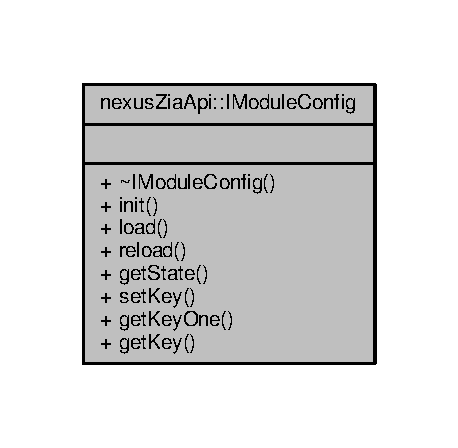
\includegraphics[width=220pt]{classnexusZiaApi_1_1IModuleConfig__coll__graph}
\end{center}
\end{figure}
\subsection*{Public Types}
\begin{DoxyCompactItemize}
\item 
enum \hyperlink{classnexusZiaApi_1_1IModuleConfig_af31b1666dea53f8776c7399e6df9e865}{State} \{ {\bfseries U\+N\+L\+O\+A\+D\+ED} = 0, 
{\bfseries L\+O\+A\+D\+\_\+\+S\+T\+A\+RT} = 1, 
{\bfseries L\+O\+A\+D\+ED} = 2, 
{\bfseries E\+R\+R\+OR} = 3
 \}
\end{DoxyCompactItemize}
\subsection*{Public Member Functions}
\begin{DoxyCompactItemize}
\item 
virtual void \hyperlink{classnexusZiaApi_1_1IModuleConfig_ac41aad2c35f3634e0bb23e4e55e1f8b8}{init} (void)=0
\item 
virtual void \hyperlink{classnexusZiaApi_1_1IModuleConfig_a9b1efedd95b96b2e019470a89370997a}{load} (void)=0
\item 
virtual void \hyperlink{classnexusZiaApi_1_1IModuleConfig_a9171887da472d0d4c9ee237ed9d1d754}{reload} (void)=0
\item 
virtual const \hyperlink{classnexusZiaApi_1_1IModuleConfig_af31b1666dea53f8776c7399e6df9e865}{State} \& \hyperlink{classnexusZiaApi_1_1IModuleConfig_a4e54fa1883c81395351091150b3aefb4}{get\+State} (void)=0
\item 
virtual void \hyperlink{classnexusZiaApi_1_1IModuleConfig_a26b6b940d232e699a405ad588ffab040}{set\+Key} (const std\+::string \&key, const \hyperlink{classnexusZiaApi_1_1IConfigKey}{I\+Config\+Key} \&config\+Key)=0
\item 
virtual const \hyperlink{classnexusZiaApi_1_1IConfigKey}{I\+Config\+Key} \& \hyperlink{classnexusZiaApi_1_1IModuleConfig_a417a022a19e631ebdc360cc5d06c91d2}{get\+Key\+One} (const std\+::string \&key)=0
\item 
virtual const std\+::list$<$ \hyperlink{classnexusZiaApi_1_1IConfigKey}{I\+Config\+Key} $>$ \& \hyperlink{classnexusZiaApi_1_1IModuleConfig_a277c40a0589820ac67f3c33bfa8a79da}{get\+Key} (const std\+::string \&key)=0
\end{DoxyCompactItemize}


\subsection{Member Enumeration Documentation}
\index{nexus\+Zia\+Api\+::\+I\+Module\+Config@{nexus\+Zia\+Api\+::\+I\+Module\+Config}!State@{State}}
\index{State@{State}!nexus\+Zia\+Api\+::\+I\+Module\+Config@{nexus\+Zia\+Api\+::\+I\+Module\+Config}}
\subsubsection[{\texorpdfstring{State}{State}}]{\setlength{\rightskip}{0pt plus 5cm}enum {\bf nexus\+Zia\+Api\+::\+I\+Module\+Config\+::\+State}\hspace{0.3cm}{\ttfamily [strong]}}\hypertarget{classnexusZiaApi_1_1IModuleConfig_af31b1666dea53f8776c7399e6df9e865}{}\label{classnexusZiaApi_1_1IModuleConfig_af31b1666dea53f8776c7399e6df9e865}
State of config loading 

\subsection{Member Function Documentation}
\index{nexus\+Zia\+Api\+::\+I\+Module\+Config@{nexus\+Zia\+Api\+::\+I\+Module\+Config}!get\+Key@{get\+Key}}
\index{get\+Key@{get\+Key}!nexus\+Zia\+Api\+::\+I\+Module\+Config@{nexus\+Zia\+Api\+::\+I\+Module\+Config}}
\subsubsection[{\texorpdfstring{get\+Key(const std\+::string \&key)=0}{getKey(const std::string &key)=0}}]{\setlength{\rightskip}{0pt plus 5cm}virtual const std\+::list$<${\bf I\+Config\+Key}$>$\& nexus\+Zia\+Api\+::\+I\+Module\+Config\+::get\+Key (
\begin{DoxyParamCaption}
\item[{const std\+::string \&}]{key}
\end{DoxyParamCaption}
)\hspace{0.3cm}{\ttfamily [pure virtual]}}\hypertarget{classnexusZiaApi_1_1IModuleConfig_a277c40a0589820ac67f3c33bfa8a79da}{}\label{classnexusZiaApi_1_1IModuleConfig_a277c40a0589820ac67f3c33bfa8a79da}
Get list of key in config of module 
\begin{DoxyParams}{Parameters}
{\em key} & \\
\hline
\end{DoxyParams}
\begin{DoxyReturn}{Returns}
std\+::list$<$\+I\+Configkey$>$ 
\end{DoxyReturn}
\index{nexus\+Zia\+Api\+::\+I\+Module\+Config@{nexus\+Zia\+Api\+::\+I\+Module\+Config}!get\+Key\+One@{get\+Key\+One}}
\index{get\+Key\+One@{get\+Key\+One}!nexus\+Zia\+Api\+::\+I\+Module\+Config@{nexus\+Zia\+Api\+::\+I\+Module\+Config}}
\subsubsection[{\texorpdfstring{get\+Key\+One(const std\+::string \&key)=0}{getKeyOne(const std::string &key)=0}}]{\setlength{\rightskip}{0pt plus 5cm}virtual const {\bf I\+Config\+Key}\& nexus\+Zia\+Api\+::\+I\+Module\+Config\+::get\+Key\+One (
\begin{DoxyParamCaption}
\item[{const std\+::string \&}]{key}
\end{DoxyParamCaption}
)\hspace{0.3cm}{\ttfamily [pure virtual]}}\hypertarget{classnexusZiaApi_1_1IModuleConfig_a417a022a19e631ebdc360cc5d06c91d2}{}\label{classnexusZiaApi_1_1IModuleConfig_a417a022a19e631ebdc360cc5d06c91d2}
Get key unique in config of module 
\begin{DoxyParams}{Parameters}
{\em key} & \\
\hline
\end{DoxyParams}
\begin{DoxyReturn}{Returns}
const \hyperlink{classnexusZiaApi_1_1IConfigKey}{I\+Config\+Key} \& 
\end{DoxyReturn}
\index{nexus\+Zia\+Api\+::\+I\+Module\+Config@{nexus\+Zia\+Api\+::\+I\+Module\+Config}!get\+State@{get\+State}}
\index{get\+State@{get\+State}!nexus\+Zia\+Api\+::\+I\+Module\+Config@{nexus\+Zia\+Api\+::\+I\+Module\+Config}}
\subsubsection[{\texorpdfstring{get\+State(void)=0}{getState(void)=0}}]{\setlength{\rightskip}{0pt plus 5cm}virtual const {\bf State}\& nexus\+Zia\+Api\+::\+I\+Module\+Config\+::get\+State (
\begin{DoxyParamCaption}
\item[{void}]{}
\end{DoxyParamCaption}
)\hspace{0.3cm}{\ttfamily [pure virtual]}}\hypertarget{classnexusZiaApi_1_1IModuleConfig_a4e54fa1883c81395351091150b3aefb4}{}\label{classnexusZiaApi_1_1IModuleConfig_a4e54fa1883c81395351091150b3aefb4}
Get state of module config In loading, is load, error in config, etc \begin{DoxyReturn}{Returns}

\end{DoxyReturn}
\index{nexus\+Zia\+Api\+::\+I\+Module\+Config@{nexus\+Zia\+Api\+::\+I\+Module\+Config}!init@{init}}
\index{init@{init}!nexus\+Zia\+Api\+::\+I\+Module\+Config@{nexus\+Zia\+Api\+::\+I\+Module\+Config}}
\subsubsection[{\texorpdfstring{init(void)=0}{init(void)=0}}]{\setlength{\rightskip}{0pt plus 5cm}virtual void nexus\+Zia\+Api\+::\+I\+Module\+Config\+::init (
\begin{DoxyParamCaption}
\item[{void}]{}
\end{DoxyParamCaption}
)\hspace{0.3cm}{\ttfamily [pure virtual]}}\hypertarget{classnexusZiaApi_1_1IModuleConfig_ac41aad2c35f3634e0bb23e4e55e1f8b8}{}\label{classnexusZiaApi_1_1IModuleConfig_ac41aad2c35f3634e0bb23e4e55e1f8b8}
Init config of module Default value of each key, etc \index{nexus\+Zia\+Api\+::\+I\+Module\+Config@{nexus\+Zia\+Api\+::\+I\+Module\+Config}!load@{load}}
\index{load@{load}!nexus\+Zia\+Api\+::\+I\+Module\+Config@{nexus\+Zia\+Api\+::\+I\+Module\+Config}}
\subsubsection[{\texorpdfstring{load(void)=0}{load(void)=0}}]{\setlength{\rightskip}{0pt plus 5cm}virtual void nexus\+Zia\+Api\+::\+I\+Module\+Config\+::load (
\begin{DoxyParamCaption}
\item[{void}]{}
\end{DoxyParamCaption}
)\hspace{0.3cm}{\ttfamily [pure virtual]}}\hypertarget{classnexusZiaApi_1_1IModuleConfig_a9b1efedd95b96b2e019470a89370997a}{}\label{classnexusZiaApi_1_1IModuleConfig_a9b1efedd95b96b2e019470a89370997a}
Load config of module \index{nexus\+Zia\+Api\+::\+I\+Module\+Config@{nexus\+Zia\+Api\+::\+I\+Module\+Config}!reload@{reload}}
\index{reload@{reload}!nexus\+Zia\+Api\+::\+I\+Module\+Config@{nexus\+Zia\+Api\+::\+I\+Module\+Config}}
\subsubsection[{\texorpdfstring{reload(void)=0}{reload(void)=0}}]{\setlength{\rightskip}{0pt plus 5cm}virtual void nexus\+Zia\+Api\+::\+I\+Module\+Config\+::reload (
\begin{DoxyParamCaption}
\item[{void}]{}
\end{DoxyParamCaption}
)\hspace{0.3cm}{\ttfamily [pure virtual]}}\hypertarget{classnexusZiaApi_1_1IModuleConfig_a9171887da472d0d4c9ee237ed9d1d754}{}\label{classnexusZiaApi_1_1IModuleConfig_a9171887da472d0d4c9ee237ed9d1d754}
Reload config of module \index{nexus\+Zia\+Api\+::\+I\+Module\+Config@{nexus\+Zia\+Api\+::\+I\+Module\+Config}!set\+Key@{set\+Key}}
\index{set\+Key@{set\+Key}!nexus\+Zia\+Api\+::\+I\+Module\+Config@{nexus\+Zia\+Api\+::\+I\+Module\+Config}}
\subsubsection[{\texorpdfstring{set\+Key(const std\+::string \&key, const I\+Config\+Key \&config\+Key)=0}{setKey(const std::string &key, const IConfigKey &configKey)=0}}]{\setlength{\rightskip}{0pt plus 5cm}virtual void nexus\+Zia\+Api\+::\+I\+Module\+Config\+::set\+Key (
\begin{DoxyParamCaption}
\item[{const std\+::string \&}]{key, }
\item[{const {\bf I\+Config\+Key} \&}]{config\+Key}
\end{DoxyParamCaption}
)\hspace{0.3cm}{\ttfamily [pure virtual]}}\hypertarget{classnexusZiaApi_1_1IModuleConfig_a26b6b940d232e699a405ad588ffab040}{}\label{classnexusZiaApi_1_1IModuleConfig_a26b6b940d232e699a405ad588ffab040}

\begin{DoxyParams}{Parameters}
{\em key} & \\
\hline
{\em config\+Key} & \\
\hline
\end{DoxyParams}
\begin{DoxyReturn}{Returns}

\end{DoxyReturn}


The documentation for this class was generated from the following file\+:\begin{DoxyCompactItemize}
\item 
/home/convly/delivery/cpp\+\_\+zia\+\_\+api/src/\+Config/Config.\+hpp\end{DoxyCompactItemize}

\hypertarget{classnexusZiaApi_1_1IModuleCore}{}\section{nexus\+Zia\+Api\+:\+:I\+Module\+Core Class Reference}
\label{classnexusZiaApi_1_1IModuleCore}\index{nexus\+Zia\+Api\+::\+I\+Module\+Core@{nexus\+Zia\+Api\+::\+I\+Module\+Core}}


Collaboration diagram for nexus\+Zia\+Api\+:\+:I\+Module\+Core\+:\nopagebreak
\begin{figure}[H]
\begin{center}
\leavevmode
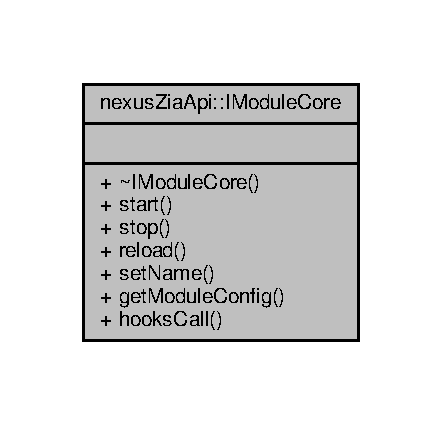
\includegraphics[width=212pt]{classnexusZiaApi_1_1IModuleCore__coll__graph}
\end{center}
\end{figure}
\subsection*{Public Types}
\begin{DoxyCompactItemize}
\item 
enum \hyperlink{classnexusZiaApi_1_1IModuleCore_abc0dcb61041187581a512822e934bc25}{State} \{ {\bfseries O\+FF} = 0, 
{\bfseries UP} = 1
 \}
\end{DoxyCompactItemize}
\subsection*{Public Member Functions}
\begin{DoxyCompactItemize}
\item 
virtual void \hyperlink{classnexusZiaApi_1_1IModuleCore_ae52fea1f96d8954f0b128a66405d4a45}{start} (void)=0
\item 
virtual void \hyperlink{classnexusZiaApi_1_1IModuleCore_ad47e9254ca0dcbe6cfcc5756ab8a1b87}{stop} (void)=0
\item 
virtual void \hyperlink{classnexusZiaApi_1_1IModuleCore_a36b1740f097ba13db39431f1c5f9f8a9}{reload} (void)=0
\item 
virtual void \hyperlink{classnexusZiaApi_1_1IModuleCore_a5770e4c73d8964916d7e429482b52e72}{set\+Name} (const std\+::string \&name)=0
\item 
virtual const \hyperlink{classnexusZiaApi_1_1IModuleConfig}{I\+Module\+Config} \& \hyperlink{classnexusZiaApi_1_1IModuleCore_a953c7450755ba4953251029980084a6c}{get\+Module\+Config} (void)=0
\item 
virtual void \hyperlink{classnexusZiaApi_1_1IModuleCore_a32cce7b43a738e457b1e436c119cd489}{hooks\+Call} (const \hyperlink{classnexusZiaApi_1_1IHooks_ab414a80fd9ed1c967916942ec5c20433}{I\+Hooks\+::\+Types} \&hooks\+Type, \hyperlink{classnexusZiaApi_1_1IHttpData}{I\+Http\+Data} \&data)=0
\end{DoxyCompactItemize}


\subsection{Member Enumeration Documentation}
\index{nexus\+Zia\+Api\+::\+I\+Module\+Core@{nexus\+Zia\+Api\+::\+I\+Module\+Core}!State@{State}}
\index{State@{State}!nexus\+Zia\+Api\+::\+I\+Module\+Core@{nexus\+Zia\+Api\+::\+I\+Module\+Core}}
\subsubsection[{\texorpdfstring{State}{State}}]{\setlength{\rightskip}{0pt plus 5cm}enum {\bf nexus\+Zia\+Api\+::\+I\+Module\+Core\+::\+State}\hspace{0.3cm}{\ttfamily [strong]}}\hypertarget{classnexusZiaApi_1_1IModuleCore_abc0dcb61041187581a512822e934bc25}{}\label{classnexusZiaApi_1_1IModuleCore_abc0dcb61041187581a512822e934bc25}
State of module loading 0\+: O\+FF / 1\+: UP 

\subsection{Member Function Documentation}
\index{nexus\+Zia\+Api\+::\+I\+Module\+Core@{nexus\+Zia\+Api\+::\+I\+Module\+Core}!get\+Module\+Config@{get\+Module\+Config}}
\index{get\+Module\+Config@{get\+Module\+Config}!nexus\+Zia\+Api\+::\+I\+Module\+Core@{nexus\+Zia\+Api\+::\+I\+Module\+Core}}
\subsubsection[{\texorpdfstring{get\+Module\+Config(void)=0}{getModuleConfig(void)=0}}]{\setlength{\rightskip}{0pt plus 5cm}virtual const {\bf I\+Module\+Config}\& nexus\+Zia\+Api\+::\+I\+Module\+Core\+::get\+Module\+Config (
\begin{DoxyParamCaption}
\item[{void}]{}
\end{DoxyParamCaption}
)\hspace{0.3cm}{\ttfamily [pure virtual]}}\hypertarget{classnexusZiaApi_1_1IModuleCore_a953c7450755ba4953251029980084a6c}{}\label{classnexusZiaApi_1_1IModuleCore_a953c7450755ba4953251029980084a6c}
Get module config \begin{DoxyReturn}{Returns}
const \hyperlink{classnexusZiaApi_1_1IModuleConfig}{I\+Module\+Config} 
\end{DoxyReturn}
\index{nexus\+Zia\+Api\+::\+I\+Module\+Core@{nexus\+Zia\+Api\+::\+I\+Module\+Core}!hooks\+Call@{hooks\+Call}}
\index{hooks\+Call@{hooks\+Call}!nexus\+Zia\+Api\+::\+I\+Module\+Core@{nexus\+Zia\+Api\+::\+I\+Module\+Core}}
\subsubsection[{\texorpdfstring{hooks\+Call(const I\+Hooks\+::\+Types \&hooks\+Type, I\+Http\+Data \&data)=0}{hooksCall(const IHooks::Types &hooksType, IHttpData &data)=0}}]{\setlength{\rightskip}{0pt plus 5cm}virtual void nexus\+Zia\+Api\+::\+I\+Module\+Core\+::hooks\+Call (
\begin{DoxyParamCaption}
\item[{const {\bf I\+Hooks\+::\+Types} \&}]{hooks\+Type, }
\item[{{\bf I\+Http\+Data} \&}]{data}
\end{DoxyParamCaption}
)\hspace{0.3cm}{\ttfamily [pure virtual]}}\hypertarget{classnexusZiaApi_1_1IModuleCore_a32cce7b43a738e457b1e436c119cd489}{}\label{classnexusZiaApi_1_1IModuleCore_a32cce7b43a738e457b1e436c119cd489}
Function call if event in the hook subsribe 
\begin{DoxyParams}{Parameters}
{\em hooks\+Type} & Type of hook \\
\hline
{\em data} & Data http \\
\hline
\end{DoxyParams}
\index{nexus\+Zia\+Api\+::\+I\+Module\+Core@{nexus\+Zia\+Api\+::\+I\+Module\+Core}!reload@{reload}}
\index{reload@{reload}!nexus\+Zia\+Api\+::\+I\+Module\+Core@{nexus\+Zia\+Api\+::\+I\+Module\+Core}}
\subsubsection[{\texorpdfstring{reload(void)=0}{reload(void)=0}}]{\setlength{\rightskip}{0pt plus 5cm}virtual void nexus\+Zia\+Api\+::\+I\+Module\+Core\+::reload (
\begin{DoxyParamCaption}
\item[{void}]{}
\end{DoxyParamCaption}
)\hspace{0.3cm}{\ttfamily [pure virtual]}}\hypertarget{classnexusZiaApi_1_1IModuleCore_a36b1740f097ba13db39431f1c5f9f8a9}{}\label{classnexusZiaApi_1_1IModuleCore_a36b1740f097ba13db39431f1c5f9f8a9}
Reload module

Module is not stop and restart, module is always UP \index{nexus\+Zia\+Api\+::\+I\+Module\+Core@{nexus\+Zia\+Api\+::\+I\+Module\+Core}!set\+Name@{set\+Name}}
\index{set\+Name@{set\+Name}!nexus\+Zia\+Api\+::\+I\+Module\+Core@{nexus\+Zia\+Api\+::\+I\+Module\+Core}}
\subsubsection[{\texorpdfstring{set\+Name(const std\+::string \&name)=0}{setName(const std::string &name)=0}}]{\setlength{\rightskip}{0pt plus 5cm}virtual void nexus\+Zia\+Api\+::\+I\+Module\+Core\+::set\+Name (
\begin{DoxyParamCaption}
\item[{const std\+::string \&}]{name}
\end{DoxyParamCaption}
)\hspace{0.3cm}{\ttfamily [pure virtual]}}\hypertarget{classnexusZiaApi_1_1IModuleCore_a5770e4c73d8964916d7e429482b52e72}{}\label{classnexusZiaApi_1_1IModuleCore_a5770e4c73d8964916d7e429482b52e72}
Set name of module 
\begin{DoxyParams}{Parameters}
{\em name} & Name of module \\
\hline
\end{DoxyParams}
\index{nexus\+Zia\+Api\+::\+I\+Module\+Core@{nexus\+Zia\+Api\+::\+I\+Module\+Core}!start@{start}}
\index{start@{start}!nexus\+Zia\+Api\+::\+I\+Module\+Core@{nexus\+Zia\+Api\+::\+I\+Module\+Core}}
\subsubsection[{\texorpdfstring{start(void)=0}{start(void)=0}}]{\setlength{\rightskip}{0pt plus 5cm}virtual void nexus\+Zia\+Api\+::\+I\+Module\+Core\+::start (
\begin{DoxyParamCaption}
\item[{void}]{}
\end{DoxyParamCaption}
)\hspace{0.3cm}{\ttfamily [pure virtual]}}\hypertarget{classnexusZiaApi_1_1IModuleCore_ae52fea1f96d8954f0b128a66405d4a45}{}\label{classnexusZiaApi_1_1IModuleCore_ae52fea1f96d8954f0b128a66405d4a45}
Start module \index{nexus\+Zia\+Api\+::\+I\+Module\+Core@{nexus\+Zia\+Api\+::\+I\+Module\+Core}!stop@{stop}}
\index{stop@{stop}!nexus\+Zia\+Api\+::\+I\+Module\+Core@{nexus\+Zia\+Api\+::\+I\+Module\+Core}}
\subsubsection[{\texorpdfstring{stop(void)=0}{stop(void)=0}}]{\setlength{\rightskip}{0pt plus 5cm}virtual void nexus\+Zia\+Api\+::\+I\+Module\+Core\+::stop (
\begin{DoxyParamCaption}
\item[{void}]{}
\end{DoxyParamCaption}
)\hspace{0.3cm}{\ttfamily [pure virtual]}}\hypertarget{classnexusZiaApi_1_1IModuleCore_ad47e9254ca0dcbe6cfcc5756ab8a1b87}{}\label{classnexusZiaApi_1_1IModuleCore_ad47e9254ca0dcbe6cfcc5756ab8a1b87}
Stop module 

The documentation for this class was generated from the following file\+:\begin{DoxyCompactItemize}
\item 
/home/convly/delivery/cpp\+\_\+zia\+\_\+api/src/\+Core/Core.\+hpp\end{DoxyCompactItemize}

%--- End generated contents ---

% Index
\backmatter
\newpage
\phantomsection
\clearemptydoublepage
\addcontentsline{toc}{chapter}{Index}
\printindex

\end{document}
